\documentclass[brazil,times]{abnt}
\usepackage[T1]{fontenc}
\usepackage[utf8]{inputenc}
\usepackage{url}
\usepackage{graphicx}
\usepackage{amssymb}
\makeatletter
\usepackage{babel}
\makeatother

\begin{document}

\autor{Pedro Paulo Vezzá Campos \\ Daniel Moraes Huguenin \\ Antonio Rui 
Castro Junior}

\titulo{Guerra Das Universidades: \\Manual do Usuário}

\comentario{Manual de usuário do projeto desenvolvido pela Equipe Knuth
apresentado para avaliação na disciplina MAC0242, do curso de Bacharelado em
Ciência da Computação, turma 45, da Universidade de São Paulo, ministrada pelo
professor Roberto Hirata Junior.}

\instituicao{Departamento de Ciência da Computação \par Instituto de Matemática
e Estatística \par Universidade de São Paulo}

\local{São Paulo - SP, Brasil}

\data{\today}

\capa

\folhaderosto

\tableofcontents

\chapter{Introdução}
% Para o projeto da disciplina MAC0242 - Laboratório de Programação II foi
% sugerido pelo professor a implementação de um jogo com temática universitária
% aos moldes de jogos famosos, tais como \emph{Civilization} ou \emph{SimCity}
% utilizando os conceitos de Programação Orientada a Objetos (POO) vistos em aula
% , linguagem Java e um \emph{framework} de desenvolvimento de jogos,
% inicialmente a sugestão foi a utilização do PlayN \cite{}.

\textbf{Guerra das Universidades} é um jogo produzido similar ao \emph{Age of
Empires} com ambiente universitário. Tal como o jogo original ele é
\emph{singleplayer} com jogabilidade 2D. O jogador assume a posição de reitor do
campus.

O objetivo é construir estruturas básicas de uma universidade, tais como blocos
de salas de aula, bandejão, setor de esportes, dentre outros além de recrutar
novos alunos e professores para compor a nova universidade. Estas ações estão
limitadas ao orçamento da universidade, que deve ser respeitado para evitar que
problemas aconteçam no campus. Quando a universidade atingir uma quantidade
suficiente de professores e alunos com condições de bem-estar o reitor pode
ordenar um ataque a universidades vizinhas, com o objetivo de desestabilizá-las.
Ao mesmo tempo, os oponentes estão montando suas estratégias para atacá-lo.
Ganha a universidade que consiga permanecer como a única sobrevivente no jogo. 

\chapter{Panorama do Jogo}

\section{Iniciando um Novo Jogo}
\begin{figure}[htp]
\begin{center}
  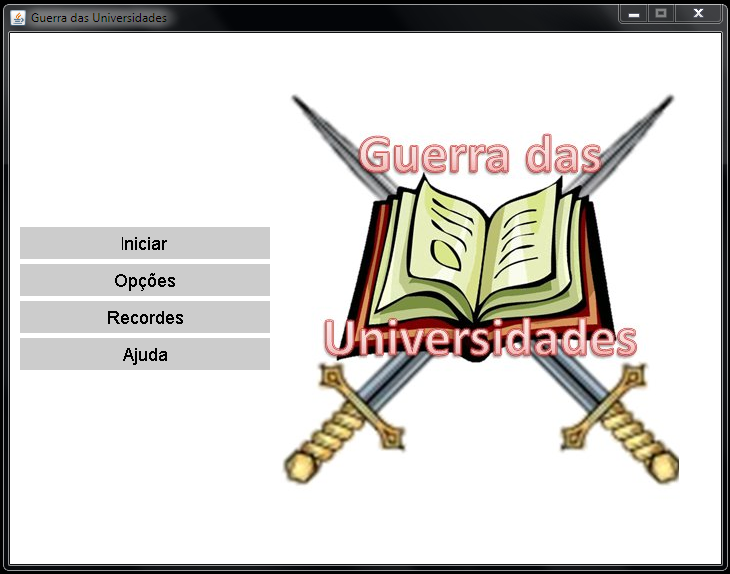
\includegraphics[width=0.6\textwidth]{img/Figura1manual.PNG}
  \caption[Tela Inicial do Jogo]{Tela Inicial do Jogo}
  \label{tela-inicial}
\end{center}
\end{figure}

No menu principal (Figura \ref{tela-inicial}), escolha Iniciar para começar o
jogo. Depois disso, você será levado a uma tela aonde escolherá seu nome e seu foco
de administraçao do mandato como reitor. Tenha em mente que cada foco de
administração acarretará em descontos no custo de estruturas e unidades
específicas. Seus efeitos serão descritos resumidamente logo abaixo de cada
foco a escolher.

\begin{figure}[htp]
\begin{center}
  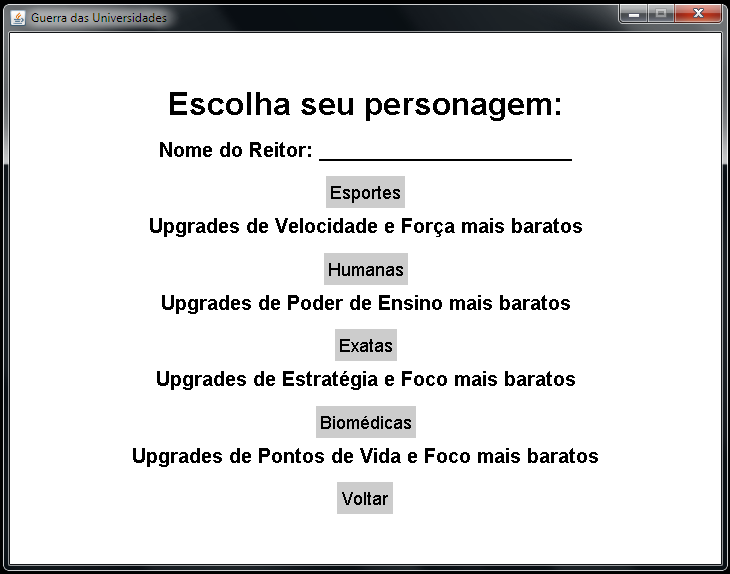
\includegraphics[width=0.6\textwidth]{img/Figura2manual.PNG}
  \caption[Escolha de Foco de Administração]{Escolha de Foco de
   Administração}
  \label{escolha-foco}
\end{center}
\end{figure}

Em seguida, você escolherá a universidade que representará
(Figura \ref{escolha-universidade}). Clique na universidade escolhida para ser
levado para a tela principal do jogo. Agora é só jogar!

\begin{figure}[htp]
\begin{center}
  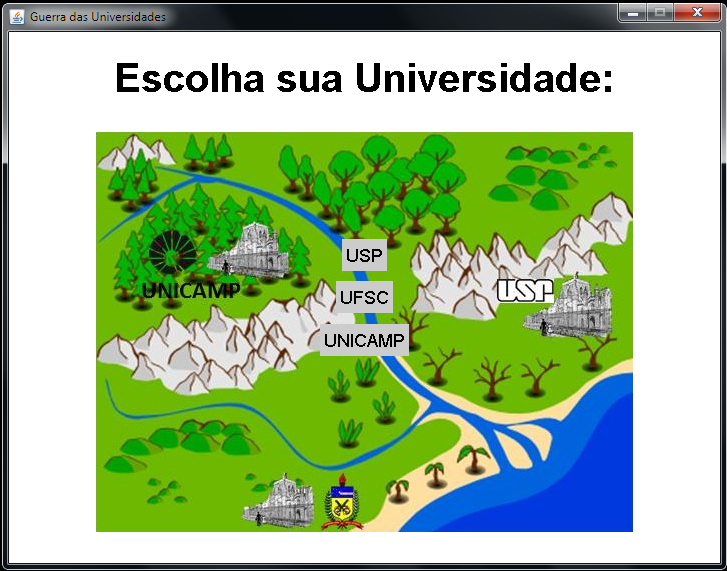
\includegraphics[width=0.6\textwidth]{img/Figura3manual.PNG}
  \caption[Escolha da Universidade]{Escolha da Universidade}
  \label{escolha-universidade}
\end{center}
\end{figure}

\section{Familiarizando-se com a Tela Principal}
	\begin{figure}[htp]
	\begin{center}
	  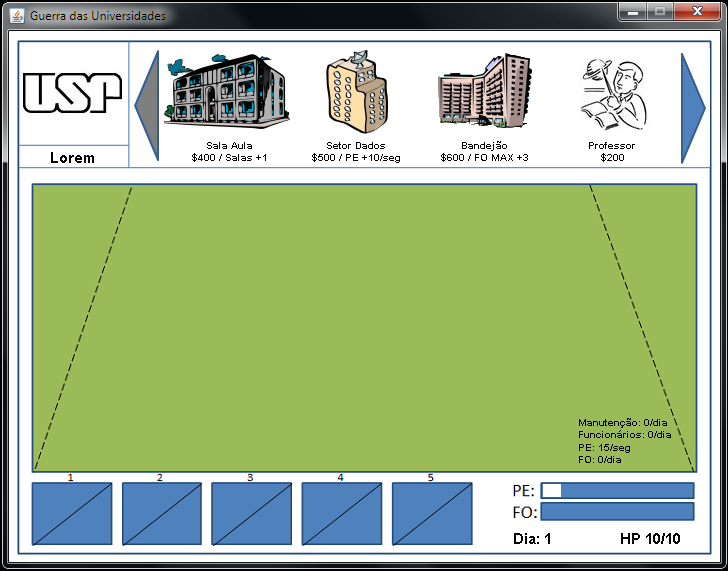
\includegraphics[width=0.8\textwidth]{img/Figura4manual.PNG}
	  \caption[Tela Principal]{TelaPrincipal}
	  \label{tela-principal}
	\end{center}
	\end{figure}

Na tela principal (Figura \ref{tela-principal}), a barra superior rola com o
clicar das setas. Nessa barra são exibidas as estruturas disponíveis para serem
construidas. Abaixo de cada estrutura é exibido seu preço e uma breve
explicação das vantagens que ela lhe fornece.

Na região central está o campus da sua universidade com todas as estruturas
compradas até o momento.

Atente que nessa tela, na parte inferior esquerda, existe uma caixa de diálogo
que mostra mensagens importantes sobre o que está acontecendo no jogo (ataque de uma
universidade por outra, ocorrência de eventos, etc). No canto direito são
exibidas suas informações de custo diário e outras informações que tem que ser
rápidas para consulta.

Na barra inferior existem 5 slots, que representam salas de aula. Inicialmente
todas as cinco salas estão indisponíveis e, à medida que você comprar as
estruturas chamadas blocos de ensino, elas vão sendo liberadas.

Ao atacar outra universidade, você poderá visualizar informações importantes,
como os pontos de vida de cada uma, Pontos de Ensino, Foco, etc. Isso é crucial
para planejar sua estratégia. A tela de visualização de oponentes (Figura
\ref{visualizar-oponentes}) pode ser acessada através de um clique em algum dos
5 slots. 

\begin{figure}[htp]
\begin{center}
  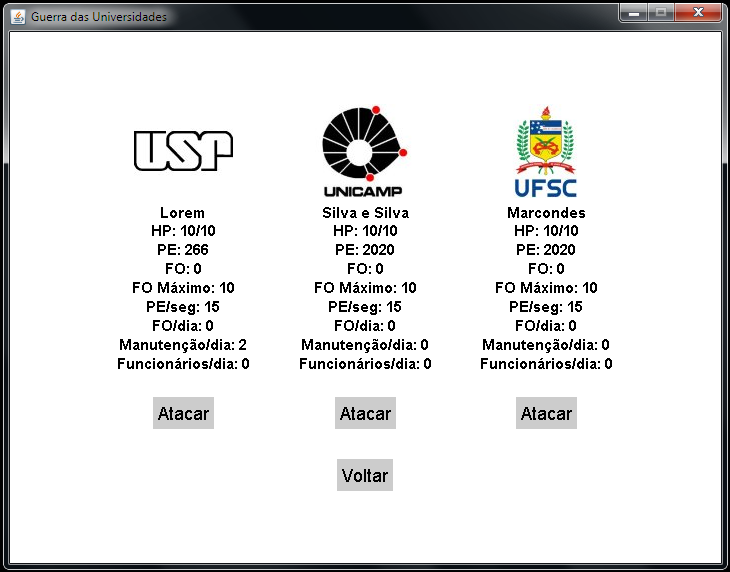
\includegraphics[width=0.8\textwidth]{img/Figura5manual.PNG}
  \caption[Visualização dos oponentes]{Visualização dos oponentes}
  \label{visualizar-oponentes}
\end{center}
\end{figure}

\chapter{Como Jogar}

\section{Pontos de PE}
No seu campus, a moeda corrente é o Poder de Ensino (PE). Com esses pontos você
pode construir novas estruturas, recrutar pessoas, matricular alunos e até
disparar eventos especiais que lhe proporcionem bonus. É fundamental
administrá-lo com sabedoria. Sua barra de PE encontra-se no canto direito
inferior, nela você pode consultar seu PE atual. Veja que inicialmente você
ganha 15 PE a cada segundo, mas essa taxa pode ser melhorada comprando algumas
estruturas e eventos.

\section{Pontos de Foco}
Os pontos de Foco determinam o ``poder'' de cada sala de aula que sai da
universidade para atacar além da capacidade de defender-se de um ataque inimigo.
Quando você manda uma sala atacar, a universidade que receber o ataque terá que
ter um foco igual ou maior do que o foco embutido na mesma, e perderá esse
valor em foco.

Caso a universidade atacada não possua foco suficiente para resistir ao ataque e
fique com um foco menor que zero, a mesma perde 1 ponto de HP (Hit Points) e
zera seu foco. No entanto, atente que não é recomendável juntar um foco grande e
muitas salas para mandar múltiplos ataques pois cada ataque diminui pela metade
seu foco atual, enfraquecendo os ataques subsequentes.

\section{Salas de Aula e Ataque}
As salas de aula são suas unidades de ataque, mas inicialmente, nenhuma sala de
aula está disponível. É necessário comprar um Bloco de Ensino para liberar cada
sala.

Depois disso, mesmo tendo uma sala de aula liberada, você só terá a
possibilidade de atacar outras universidades se tiver uma sala de aula cheia e
um foco maior que zero. Para uma sala estar cheia ela deve ter 1 professor e 10
alunos. Com a sala completa, é possivel enviá-la para atacar outra universidade
de sua escolha afim de destruí-la.

\section{Custos de Manutenção Diários, Greves e Perda de Estruturas}
Os custos de manutenção diários determinam quantos pontos de PE você gasta por
dia para manter sua universidade funcionando. No jogo, um dia são 10 segundos
(Podendo ser acelerado dependendo da dificuldade do jogo), e o dia atual é
marcado próximo aos seus pontos de PE para fácil consulta.

A cada 10 segundos um dia se passrá e se, ao final desse dia, você não possuir
PE suficiente para pagar as manutenções, determinados eventos podem ocorrer:
Haverá uma probabilidade de 3\% de funcionarios entrarem em greve (o que zera o
foco dos alunos), 3\% uma estrutura aleatória quebrar ou 4\% de chande de ambas
as coisas acontecerem, então fique atento ao seus custos diarios.

\section{Pontos de HP e Condições de Vitória ou Derrota}
Sua universidade tem pontos chamados Hit Points (HP). Quando esses pontos chegam
a zero, sua universidade será destruída e você perde o jogo. E ao atacar uma
outra universidade um número de vezes suficiente para levar sua HP a zero, você
a destruirá. Destruindo todas as outras universidades, você vencerá o jogo!

\begin{figure}[htp]
\begin{center}
  
\includegraphics[width=0.4\textwidth]{img/Figura6manual.PNG}
  \caption[Tela de Vitória]{Tela de Vitória}
  \label{tela-vitoria}
\end{center}
\end{figure}

\begin{figure}[htp]
\begin{center}
  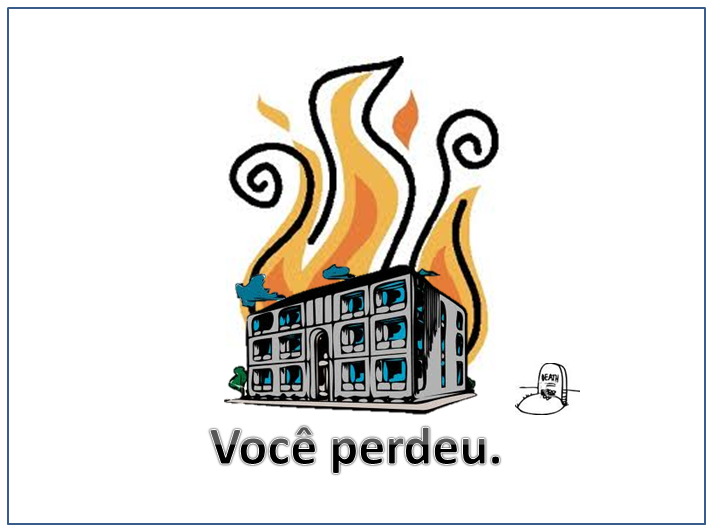
\includegraphics[width=0.4\textwidth]{img/Figura7manual.PNG}
  \caption[Tela de Derrota]{Tela de Derrota}
  \label{tela-derrota}
\end{center}
\end{figure}

\section{Recordes}
Os recordes são acessados através da tela inicial do jogo e são baseados no
tempo em que o jogador levou para vencer o jogo. Tente bater seu próprio
recorde!

\section{Dificuldade do Jogo}
Se o jogo estiver muito difícil pra você ou até mesmo pouco desafiador, acesse a
tela de opções através do Menu Inicial e regule a dificuldade do jogo.


\chapter{Incrementos Disponíveis}

\section{Estruturas}

\subsection{Bloco de Ensino}
\begin{description}
	\item[Custo]  400
	\item[Efeitos] Libera uma das 5 salas de aula
	\item[Manutenção/dia] 0
	\item[Limite] 5
	\item[Requisitos] Nenhum
\end{description}

\subsection{Bandejão}
\begin{description}
	\item[Custo]  600
	\item[Efeitos] Foco máximo passa a ser 13
	\item[Manutenção/dia] 0
	\item[Limite] 1
	\item[Requisitos] Nenhum
\end{description}

\subsection{Setor de Dados}
\begin{description}
	\item[Custo]  500
	\item[Efeitos] PE/seg + 10
	\item[Manutenção/dia] 3
	\item[Limite] 1
	\item[Requisitos] Pelo menos um bloco de ensino
\end{description}

\subsection{Praça Central}
\begin{description}
	\item[Custo]  400
	\item[Efeitos] Foco +1/dia
	\item[Manutenção/dia] 2
	\item[Limite] 1
	\item[Requisitos] Nenhum
\end{description}

\subsection{Centro de Esportes}
\begin{description}
	\item[Custo]  700
	\item[Efeitos] Foco +1/dia
	\item[Manutenção/dia] 2
	\item[Limite] 1
	\item[Requisitos] Nenhum
\end{description}

\subsection{Guarda Universitaria}
\begin{description}
	\item[Custo] 1500
	\item[Efeitos] Se a universidade é atacada e o foco fica menor que zero, essa
	estrutura é destruída, ao invés da universidade perder 1 ponto de HP
	\item[Manutenção/dia] 2
	\item[Limite] 1 durante todo o jogo, não é possível recomprar a Guarda caso
	ela seja destruída.
	\item[Requisitos] Nenhum
\end{description}

\section{Eventos}

\subsection{Aumento Salarial}
\begin{description}
	\item[Custo] 700
	\item[Efeitos] +3 PE/seg
	\item[Manutenção funcionários/dia] 2 
	\item[Limite]  10
	\item[Requisitos] Possuir pelo menos um bloco de ensino
\end{description}

\subsection{Churrasco-Debate}
\begin{description}
	\item[Custo] 400 (275, Se foco da administração for Humanas)
	\item[Efeitos] +1 PE/seg
	\item[Limite] 15
	\item[Requisitos] Nenhum
\end{description}

\subsection{Promover Festa}
\begin{description}
	\item[Custo] 400 (300, Se foco da administração for Biomédicas)
	\item[Efeitos] Foco +2 
	\item[Limite] $\infty$
	\item[Requisitos] Nenhum
\end{description}

\subsection{Sobremesa no Bandejão}
\begin{description}
	\item[Custo] 250 (140, Se foco da administração for Biomédicas)
	\item[Efeitos] Foco +1
	\item[Limite]  $\infty$
	\item[Requisitos] Possuir o Bandejão
\end{description}

\subsection{Promover Seminário}
\begin{description}
	\item[Custo] 300 (200, Se foco da administração for Exatas)
	\item[Efeitos] PE/seg +7 por 7 dias
	\item[Limite] $\infty$
	\item[Requisitos] Possuir pelo menos um bloco de ensino
\end{description}

\subsection{Contratar Professor}
\begin{description}
	\item[Custo]  200
	\item[Efeitos] Adiciona um professor a uma sala livre
	\item[Limite] A quantidade de salas abertas
	\item[Requisitos] Pelo menos uma sala aberta sem professor
\end{description}

\subsection{Matricular Aluno}
\begin{description}
	\item[Custo]  75
	\item[Efeitos] Adiciona um aluno a uma sala livre.
	\item[Limite] 10 alunos por sala aberta.
	\item[Requisitos] Pelo menos uma sala aberta e não lotada.
\end{description}


%\bibliographystyle{abnt-num}
%\bibliography{bibliografia}
\end{document}